\documentclass[
  bibliography=totoc,     % Literatur im Inhaltsverzeichnis
  captions=tableheading,  % Tabellenüberschriften
  titlepage=firstiscover, % Titelseite ist Deckblatt
]{scrartcl}

%irgendetwas mit Tabelen und Figuren anders Nummerieren 
\usepackage{chngcntr}
\usepackage{longtable} 

\usepackage{titling}

%Textdatein einfügen
\usepackage{verbatim}

% Paket float verbessern
\usepackage{scrhack}

% Warnung, falls nochmal kompiliert werden muss
\usepackage[aux]{rerunfilecheck}

% unverzichtbare Mathe-Befehle
\usepackage{amsmath}
% viele Mathe-Symbole
\usepackage{amssymb}
% Erweiterungen für amsmath
\usepackage{mathtools}

% Fonteinstellungen
\usepackage{fontspec}
% Latin Modern Fonts werden automatisch geladen
% Alternativ zum Beispiel:
%\setromanfont{Libertinus Serif}
%\setsansfont{Libertinus Sans}
%\setmonofont{Libertinus Mono}

% Wenn man andere Schriftarten gesetzt hat,
% sollte man das Seiten-Layout neu berechnen lassen
\recalctypearea{}

% deutsche Spracheinstellungen
\usepackage[ngerman]{babel}


\usepackage[
  math-style=ISO,    % ┐
  bold-style=ISO,    % │
  sans-style=italic, % │ ISO-Standard folgen
  nabla=upright,     % │
  partial=upright,   % ┘
  warnings-off={           % ┐
    mathtools-colon,       % │ unnötige Warnungen ausschalten
    mathtools-overbracket, % │
  },                       % ┘
]{unicode-math}

% traditionelle Fonts für Mathematik
\setmathfont{Latin Modern Math}
% Alternativ zum Beispiel:
%\setmathfont{Libertinus Math}

\setmathfont{XITS Math}[range={scr, bfscr}]
\setmathfont{XITS Math}[range={cal, bfcal}, StylisticSet=1]

% Zahlen und Einheiten
\usepackage[
  locale=DE,                   % deutsche Einstellungen
  separate-uncertainty=true,   % immer Unsicherheit mit \pm
  per-mode=symbol-or-fraction, % / in inline math, fraction in display math
]{siunitx}

\DeclareSIUnit{\channel}{Channel}
\DeclareSIUnit{\year}{a}

% chemische Formeln
\usepackage[
  version=4,
  math-greek=default, % ┐ mit unicode-math zusammenarbeiten
  text-greek=default, % ┘
]{mhchem}

% richtige Anführungszeichen
\usepackage[autostyle]{csquotes}

% schöne Brüche im Text
\usepackage{xfrac}

% Standardplatzierung für Floats einstellen
\usepackage{float}
\floatplacement{figure}{htbp}
\floatplacement{table}{htbp}

% Floats innerhalb einer Section halten
\usepackage[
  section, % Floats innerhalb der Section halten
  below,   % unterhalb der Section aber auf der selben Seite ist ok
]{placeins}

% Seite drehen für breite Tabellen: landscape Umgebung
\usepackage{pdflscape}

% Captions schöner machen.
\usepackage[
  labelfont=bf,        % Tabelle x: Abbildung y: ist jetzt fett
  font=small,          % Schrift etwas kleiner als Dokument
  width=0.9\textwidth, % maximale Breite einer Caption schmaler
]{caption}
% subfigure, subtable, subref
\usepackage{subcaption}

% Grafiken können eingebunden werden
\usepackage{graphicx}
\usepackage{wrapfig}

% schöne Tabellen
\usepackage{booktabs}
\usepackage[table]{xcolor}

% Verbesserungen am Schriftbild
\usepackage{microtype}

% Literaturverzeichnis
\usepackage[
  backend=biber,
  sorting=none
]{biblatex}
% Quellendatenbank
\addbibresource{lit.bib}
\addbibresource{programme.bib}

% Hyperlinks im Dokument
\usepackage[
  german,
  unicode,        % Unicode in PDF-Attributen erlauben
  pdfusetitle,    % Titel, Autoren und Datum als PDF-Attribute
  pdfcreator={},  % ┐ PDF-Attribute säubern
  pdfproducer={}, % ┘
]{hyperref}
% erweiterte Bookmarks im PDF
\usepackage{bookmark}

% Trennung von Wörtern mit Strichen
\usepackage[shortcuts]{extdash}

%\setcounter{tocdepth}{3} % + subsubsections



\author{%
  Benedikt Lütke Lanfer \\%
  \href{mailto:benedikt.luetkelanfer@tu-dortmund.de}{benedikt.luetkelanfer@tu-dortmund.de}%
  \and%
  Enno Wellmann \\%
  \href{mailto:enno.wellmann@tu-dortmund.de}{enno.wellmann@tu-dortmund.de}%
}
\publishers{TU Dortmund – Fakultät Physik}


\newcommand*\diff{\mathop{}\!\mathrm{d}}

\NewDocumentCommand \OverfullCenter {+m} {
\noindent\makebox[\linewidth]{#1} }

\usepackage{adjustbox}


% %Tabellen und Figuren Einstellung
% \counterwithout{table}{section}
% \counterwithout{figure}{section}
% \renewcommand{\thetable}{\Roman{table}}
% \renewcommand{\thefigure}{\Roman{figure}}

%Richtiges Einrücken
\setlength{\parindent}{0pt}


\title{V18:\\ Germanium Detektor}
\author{Benedikt Lütke Lanfer \and Enno Wellmann}
\date{06. Mai 2024}
\publishers{TU Dortmund – Fakultät Physik}

\begin{document}
\begin{titlingpage}
    \begin{center}
        \begin{Huge}
            \textbf{\thetitle\\}
        \end{Huge}
    \end{center}
    \vspace{4cm}
    
\includegraphics[width=\textwidth]{Bilder/Logo_TU.png} \\
    \vspace{4cm}
    \begin{center}
        \begin{huge}
            \theauthor\\
        \end{huge}
        \vspace{0.5cm}
        \begin{Large}
            benedikt.luetkelanfer@tu-dortmund.de\\
            enno.wellmann@tu-dortmund.de\\
            \vspace{1.4cm}
            Bearbeitet: \today\\
            Durchgeführt: \thedate\\
            TU Dortmund – Fakultät Physik\\
        \end{Large}
    \end{center}
\end{titlingpage}
\tableofcontents
\newpage

\section{Zielsetzung}
In diesem Versuch wird ein Germanium Energiedetektor mit einer geeichten 152Eu
Quelle kalibriert. Der kalibrierte Detektor wird anschließend verwendet um das
Spektrum einer monochromatischen 137Cs Quelle aufzunehmen. Danach wird mit dem
Spektrum einer 133Ba Quelle deren Aktivität bestimmt. Schließlich wird anhand
eines weiteren Spektrums eine unbekannte Quelle identifiziert.

% Stichworte:
% \begin{itemize}
% \item Vollenergienachweiswahrscheinlichkeit
% \item Linien des Eu Spektrums
% \item Halbwertsbreite
% \item Compton Kante \item
% \end{itemize}

%---------------------------------------------------------------------------------------------------------------------------------------------------------------%

\section{Theorie}
\subsection[]{Wechselwirkung von Strahlung mit Materie}
Die Interaktionswahrscheinlichkeit von Gamma Strahlen mit Materie lässt sich
durch den Dämpfungskoeffizienten $\mu$ darstellen. Die Strahlungsintensität
fällt in dichten Materialien exponentiell ab $I ~ \exp(-\mu x)$. Dieser
Intensitätsverlust hängt direkt mit der Wirkungsquerschnitt des materials
zusammen und ist in $\mu$ eine additive Größe. Die Dämpfungskoeffizienten von
Gammastrahlen sind in Abbildung \ref{fig:mu} zu sehen.

\begin{figure}
	\centering
	\begin{subfigure}{.5\textwidth}
		\centering
		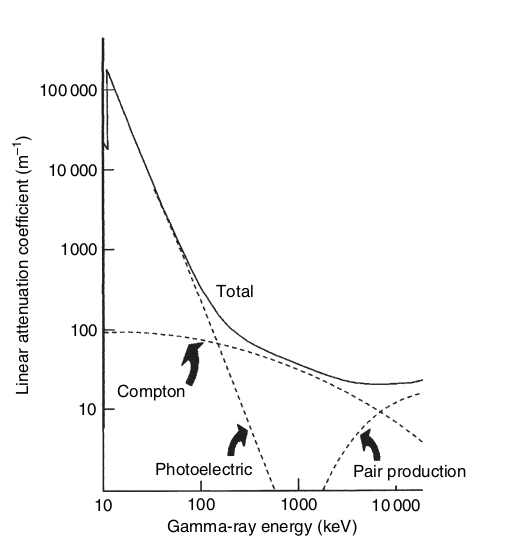
\includegraphics[width=0.9\linewidth]{./Bilder/E_mu_Gilmore.png}%
		\caption{Linearer Dämpfungskoeffizient aus \cite{book:gil}.}\label{fig:mu}
	\end{subfigure}%
	\begin{subfigure}{.5\textwidth}
		\centering
		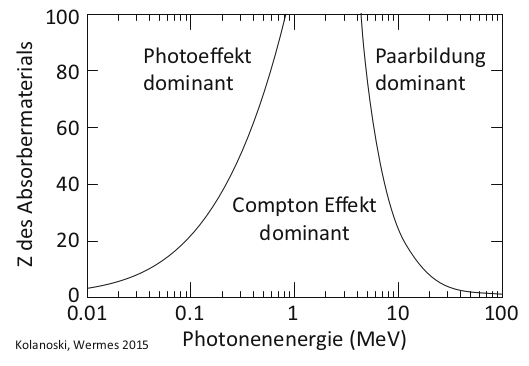
\includegraphics[width=0.9\linewidth]{./Bilder/E_Z_Kolanoski.png}
		\caption{Dominante Effekte nach $E_\gamma$ und $Z$ aus \cite{book:kolano}.}\label{fig:z}
	\end{subfigure}
	\caption{Interaktionswahrscheinlichkeiten von Gammastrahlen in verschiedenen Darstellungen.}\label{fig:zmu}
\end{figure}

Aus \cite{book:gil}. Die dominierenden Wechselwirkungen von Photonen mit
Materie sind die photoelektrische Absorption, die Compton Streuung und die
Elektronenpaarbildung. Bei der \textbf{photoelektrischen Absorption}
wechselwirkt das Photon mit einem im Atom gebundenen Elektron und befördert es
aus seinem gebundenen Zustand. Die Energie des Photons wird danach von dem
Elektron getragen und das Atom emittiert Strahlung, wenn es sich wieder abregt. Diese Interaktion
findet vor allem bei niederenergetischen Photonen statt. Eine grobe Annäherung
für das Verhalten der Wechselwirkungswahrscheinlichkeit ist der Term
\begin{align}
	\tau = \text{constant} \cdot \frac{Z^n}{E_{\gamma}^{m}}
\end{align} %TODO \tau mit dem linearen <Dämpfungskoeffizienten in Verbindung bringen.
wobei $m$ und $n$ zwischen 3 und 5 liegen \cite[vgl.][Kap 2.2.1]{book:gil}.
$\tau$ lässt sich hier in Verbindung mit dem linearen Dämpfungskoeffizienten bringen
\begin{align}
	\mu_{\text{PE}} = \tau \cdot \rho \cdot N_A /A
\end{align}

Die \textbf{Compton Streuung} ist in diesem Versuch aufgrund kleiner Energien
und großen $Z$ die häufigste Interaktion der Strahlung mit dem Material. Sie
ist (abhängig von $Z$) dominant bei Energien im Bereich von etwa
$\qtyrange{0.5}{10}{\MeV}$ Ihr differentieller Wirkungsquerschnitt wird durch die
Klein-Nishina-Formel beschrieben
\begin{align}
	\frac{d\sigma}{d \Omega} = Z r_0^2 \left(\frac{1}{1+\alpha(1-\cos\theta)}\right)^2
	\left(\frac{1+ \cos^2\theta}{2}\right)%
	\left(1+ \frac{\alpha^2(1-\cos \theta)^2}{(1+\cos^2 \theta)[1+\alpha(1-\cos(\theta))]}\right)
	\label{eq:wq_compton}
\end{align}% 
wobei $\alpha = h \nu / m_0 c²$ und $r_0$ der klassische Elektronenradius ist (vgl. \cite{book:knoll}).
Der Energieübertrag auf das Elektron wird berechnet durch
\begin{align}
	E_{e} = E_{\gamma} \left\{1- \frac{1}{1+ E_{\gamma}(1-\cos\theta)/m_0 c^2} \right\}
	\label{eq:ecompton}
\end{align}
Für diesen Versuch ist es wichtig, den Wirkungsquerschnitt der Comptonstreuung in Abhängigkeit der
Energie des gestreuten Elektrons $T = E_{\gamma} - E'_{\gamma}$ zu betrachten.
Hierfür wird in \cite[][Kap. 3.5.3]{book:kolano} die Klein-Nishina-Formel integriert.
\begin{align}
	\frac{d \sigma}{d T} =  \frac{\pi r_{e}^{2}}{m_e c^2 \epsilon}%
	\left[2 + \frac{t^2}{\epsilon^2(1-t)^2} + \frac{t}{1-t} %
		\left(t - \frac{2}{\epsilon} \right) \right]
	\label{eq:compton_energie}
\end{align}
Hier gelten $\epsilon = E_{\gamma} / (m_e c^2)$ und $t = T/ E_\gamma$.
Bei Rückstreuung des $\gamma$ Photons wird die Energie des Elektrons maximal
$T \rightarrow T_{max}$
Es ergibt sich im Spektrum die sogenannte Compton Kante bei

\begin{align}
	T_{CK}= E_\gamma \frac{2\epsilon}{1+2\epsilon}
	\label{eq:CK}
\end{align}

und der Rückstrahlpeak bei

\begin{align}
	T_{RP}= E_\gamma \frac{1}{1+2\epsilon}
	\label{eq:RP}
\end{align}

Bei Energien oberhalb der doppelten Ruhemasse des Elektrons ($\qty{1.02}{\MeV}$)
ist die \textbf{Elektronenpaarbildung} möglich. Diese Wechselwirkung tritt aber
nur bei sehr hochenergetischen Gammastrahlen auf (vgl \ref{fig:zmu}). Ihr
Wirkungsquerschnitt ist weit oberhalb der Eigenenergie konstant in $E_\gamma$
und proportional zu $Z^2$ des Absorbiermaterials \cite[vgl.][Kap
	3.5.5]{book:kolano}.

\subsection{Messung von Energie in Germanium Halbleiterdetektoren \cite{book:gil}}

Halbleiter Können durch das Bandstruktur Modell aus der Festkörperphysik
beschreiben werden. Elektronen befinden sich in einem Festkörper nicht auf
eindeutig festgelegten Energieniveaus, sondern auf Materialabhängigen
Energiebändern. Elektronen können die Energien zwischen diesen Bändern nicht
annehmen. Damit ein Strom in einem Material fließen kann, muss ein Elektron das
sogenannte Valenzband verlassen und ins Leitungsband des Materials wechseln. In
einem Halbleiter sind das Valenzband (das oberste voll besetzte Band) und das
Leitungsband durch eine Bandlücke in der Größenordnung von $\qty{1}{\eV}$
voneinander getrennt.
\begin{figure}
	\centering
	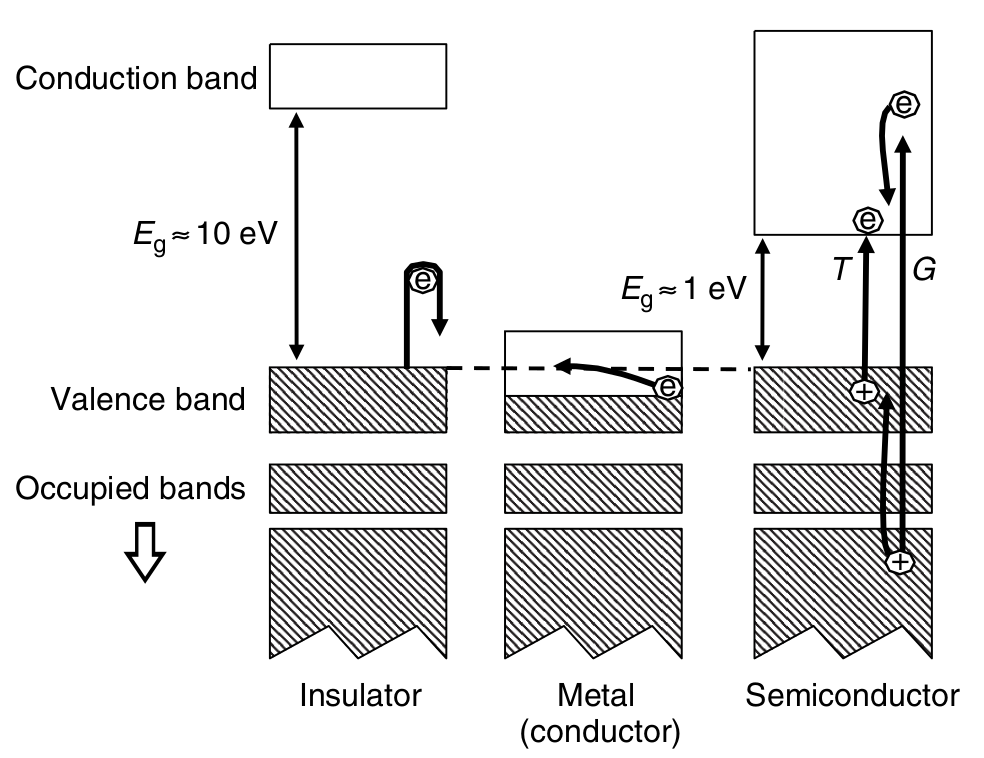
\includegraphics[width=0.4\textwidth]{./Bilder/ElectronBandsGilmore.png}
	\caption{Elektronen Bandstruktur aus \cite{book:gil}}\label{fig:eband}
\end{figure}
Das Leitungsband eines Halbleiters enthält meist auch Elektronen abhängig von
der Temperatur des Materials.
% Gleichung einfügen?
Um einen Halbleiter zu erhalten, der nach Möglichkeit nur von außen angeregte
Elektronen in seinem Leitungsband hat, ist es sinnvoll diesen so weit wie
möglich herunter zu kühlen. Gamma Strahlen erzeugen in der Interaktion mit dem
Detektor schnelle Elektronen, die durch das anregen von Bandelektronen ihre
Energie abgeben. Dieses Elektronen können in einem Germanium Halbleiter
Elektronenlochpaare erzeugen, wenn diese die notwendige Energie von $\epsilon =
	\qty{2.96}{\eV}$ erreichen. Die Anzahl an Elektronenlochpaaren ist mit
\begin{align}
	N = E_e / \epsilon
\end{align}

proportional zu der Energie $E_e$ des Elektrons. Basierend auf der Stärke des
Halbleiterstroms lassen sich so Rückschlüsse auf die Energie des Elektrons
ziehen.

\subsection{Form des Detektors \cite[vgl][Kap. 2.4]{book:gil}}

Die Größe des Detektors spielt eine wichtige Rolle darin wie die Energie des
$\gamma$ Photons in ein Spektrum von Elektronenenergien übersetzt wird. Für die
moderat Energiereichen $\gamma$ Strahlen werden für diese Diskussion nur der
Compton Effekt und die photoelektrische Absorption beachtet. In einem
idealisierten kleinen Detektor streuen die $\gamma$ Photonen nur einmal und
geben dabei entweder ihre gesamte Energie an ein Photoelektron oder einen Teil
der Energie an ein Compton gestreutes Elektron. Compton gestreuten
Gammastrahlen hinterlassen nur einen teil ihrer Energie in dem Germanium
Detektor, und verlassen diesen direkt danach wieder. Das Ergebnis ist ein
Spektrum in der Form des Compton Wirkungsquerschnitts $d\sigma/dN$ aus
Gleichung \eqref{eq:compton_energie}. Bei einem realistischen Detektor können
die Compton gestreuten Photonen im Prinzip noch weitere male mit dem Detektor
interagieren und so eine Elektronenenergie zwischen dem Vollenergiepeak und dem
erwarteten wert im Compton Kontinuum erreichen.

\subsection{Dateninterpretation}

Die Quellen werden mit einem festen Abstand $d$ zum zylinderförmigen Detektor
mit Radius $r$ eingespannt. Sie strahlen gleichmäßig in alle Richtungen ab
können aber nur im Kegelförmigen Raumwinkel des Detektors gemessen werden. Ist
$2\theta$ der Öffnungswinkel des Kegels so ist \cite{wiki:raum}
\begin{align}
	\Omega = 4 \pi sin^2\left(\frac{\theta}{2}\right) \\
	\theta = \arctan \left(\frac{r}{d} \right)
\end{align}\label{eq:raumwinkel}

Die Anzahl $Z$ an Messungen in einem bestimmten Energiepeak hängt von dem
Raumwinkel $\Omega$, der Emissionswahrscheinlichkeit $W$, der Aktivität $A$ und
der Vollenergienachweiswahrscheinlichkeit $Q$ ab. Die
Vollenergienachweiswahrscheinlichkeit ist eine wichtige Kenngröße des
Detektors. Sie ist das Verhältnis von Photoelektrisch absorbierten
Gammastrahlen, die ihre Energie vollständig abgeben und z.B. Compton gestreuten
Elektronen, die die Energie nur teilweise abgeben.
\begin{align}
	Z = \frac{\Omega}{4\pi} A T W Q
	\label{eq:Q}
\end{align}

Die entstehenden Peaks sind Poisson verteilt. Für große N können die
Histogramme aber mit einer Gaußverteilung angenähert werden. Bei den Peaks
lässt sich die Zehntelwertsbreite und die Halbwertsbreite bestimmen. Wenn es
sich bei diesen um gaußverteilte Werte handelt haben sie eine Halbwertsbreite
von $2\sqrt{2\ln 2} \sigma$ und eine Zehntelwertsbreite von $2 \sqrt{2\ln10}\sigma$.

% \subsection{Wahrscheinlichste Photonenenergien}

% \begin{itemize}
% 	\item[\ce   {^{152}Eu}] - \qty{ 40.1186 } {\keV} \qty{37.7 (5)}{\%}
% 	\item[\ce   {^{152}Eu}] - \qty{121.7817 (3)} {\keV} \qty{28.41 (13)}{\%}
% 	\item[\ce   {^{152}Eu}] - \qty{344.2785 (12)} {\keV} \qty{26.59 (12)}{\%}
% 	\item[\ce   {^{137}Cs}] - \qty{661.6553 (30)} {\keV} \qty{85.01 (20)}{\%}
% 	\item[\ce   {^{133}Ba}] - \qty{30.9731}{\keV} \qty{62.4 (7)}{\%} x ray peak
% 	\item[\ce   {^{133}Ba}] - \qty{356.0129 (7)}{\keV} \qty{62.05 (19) 	}{\%} breiterer peak
% 	\item[\ce   {^{125}Sb}] - \qty{427.88}{\keV} \qty{29.6}{\%}
% \end{itemize}
% \cite{web:lara}

\newpage
\subsection{Fehlerrechnung}
Für die Fehlerrechnung werden alle \textbf{Mittelwerte} von $N$ Messungen
folgendermaßen berechnet:

\begin{equation}
	\overline{x} = \frac{1}{N} \cdot \sum_{i=1}^N x_i
	\label{eqn:Mittelwert}
\end{equation}

und alle \textbf{Standardabweichungen zum Mittelwert} mit:

\begin{equation}
	\increment\overline{x} = \sqrt{\frac{1}{N\cdot(N-1)}\cdot\sum_{i=1}^N (x_i-\overline{x})^2}
	\label{eqn:St_Mittelwert}
\end{equation}

Bei einigen Messungen bzw Messdaten ist der Fehler auch schon im Vorhinein
angegeben. Der Fehler für zusammenhängende Messwerte wird dann mit der
\textbf{Gaußschen Fehlerfortpflanzung} berechnet:

\begin{equation}
	\increment{f} = \sqrt{ \sum_{i = 1}^{N}  \biggl(\frac{\partial{f}}{\partial{x_i}}\biggr)^2\cdot(\increment{x_i})^2}
	\label{eqn:Gauss}
\end{equation}

Die Fehlerfortpflanzung wird mit Uncertainties in Python \cite{uncertainties}
ermittelt.

%---------------------------------------------------------------------------------------------------------------------------------------------------------------%

\section{Durchführung \cite[vgl.][]{man:v18}}

Der hier verwendete Detektor ist Zylinderförmig (l= \qty{39}{\mm}, Durchmesser
= \qty{45}{\mm}) und befindet sich in einer Aluminium Schutzhülle. Der Abstand
des Detektors zur Schutzhülle beträgt \qty{1.5}{\cm}. Die Schutzhülle sorgt
dafür, dass Gammastrahlen mit einer Energie niedriger als etwa
\qtyrange{40}{50}{\keV} nicht gemessen werden können. Für die
Vollenergienachweiswahrscheinlichkeit werden nur Energien größer
\qty{150}{\keV} betrachtet. Im Inneren des Detektors befindet sich eine
Koaxiale Bohrung deren innere Oberfläche mit Gold bedampft ist. Dieser Metall
Kontakt sorgt für die Ausprägung einer Verarmungszone in dem Detektor, die
diesen zu einem effektiven Halbleiter macht.

\begin{figure}
	\centering
	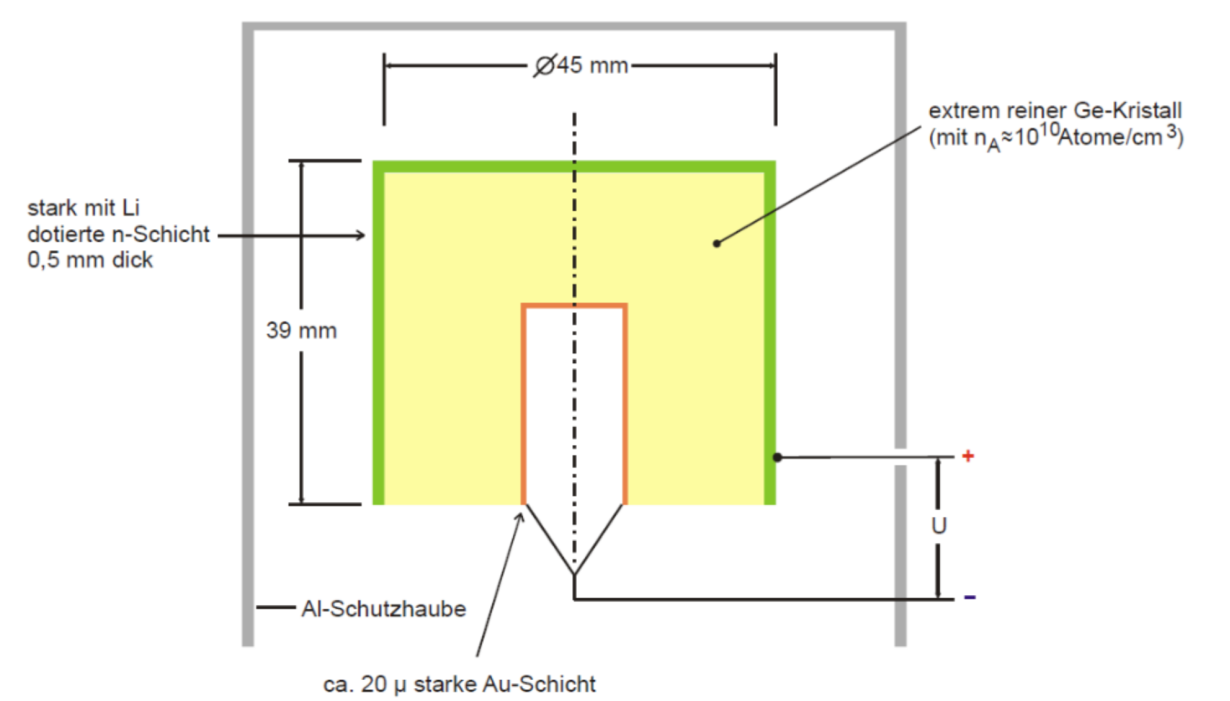
\includegraphics[width=0.4\textwidth]{./Bilder/querschnitt_detektor.png}
	\caption{Querschnitt des Germanium Detektors}\label{fig:cross}
\end{figure}

% TODO Abmessungen fertig machen

\subsection{Elektronik \cite[][Kap.17]{book:kolano}}
Der Detektor wird in diesem Versuchsaufbau durch vorgefertigte Bauteile
kontrolliert und ausgelesen. Ein Temperaturwächter kontrolliert die Kühlung des
Detektors und hält dessen Temperatur konstant auf $\qty{77}{\kelvin}$. Eine
Hochspannungsquelle erhält die Verarmungszone des Halbleiters aufrecht.
Um die Signale mit dem im PC eingebauten Viel-Kanal-Analysator detektieren können, 
müssen diese erst Analog verarbeitet und verstärkt werden. 
Dabei geht man hier wie folgt vor:

\begin{figure}
	\centering
	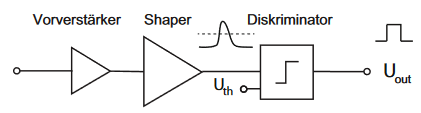
\includegraphics[width=0.8\textwidth]{./Bilder/Elektronik.png}
	\caption{Verarbeitungselektronik \cite{book:kolano}}\label{fig:elek}
\end{figure}

\begin{enumerate}
	\item \textbf{Vorverstärker:} Dieser verstärkt die Amplitude des gemessenen Signals, welches meist nur im Nanoampere Bereich ist. 
	\item \textbf{Der Shaper} verhindert die Überlagerung von Signal-Pulsen ($pile-up$) und verringert das Hintergrundrauschen. 
	Diese $pile-up$ können am Ausgang des Vorverstärkers entstehen, wenn ein weiteres Signal während seiner Abklingzeit eintritt.
	Durch eine Reihe von Hoch-/Tiefpässen können so die $pile-up$ in gaußförmige Pulse umgeformt ($shapen$) werden.
	Dieser Effekt wird im einfachsten Fall durch eine Reduzierung der Bandbreite der Signale erreicht.   
	\item \textbf{Diskriminator:} Um das Signal vom Rauschen zu filtern, wird ein Diskriminator eingesezt, welcher 
	die Signale oberhalb eines bestimmten Schwellwerts ($threshold$) durchlässt.
	Überschreitet das Signal diesen Schwellwert wird ein logisches Signal erzeugt. 
	Dies kann als Trigger für den Multichannel Analyzer verwendet werden.
	Auf diese Weise wird das weniger starke Hintergrundsignal herausgefiltert. 
\end{enumerate}

Diese Signale werden dann dem Computer übergeben, der mittels eines Viel-Kanal-Analysator ein Histogramm mit Zählrate in Abhängig vom Kanal erstellt.
Diese Kanäle müssen dann in der Auswertung, mittels des $\ce{^{152}Eu}$-Spektrums, nach der Energie Kalibriert werden.  

\subsection{Messprogramm}
Die Energiespektren von $\ce{^{152}Eu}$, der $\ce{^{137}Cs}$ und $\ce{^{133}Ba}$ werden
aufgenommen. Hierzu werden die Proben in einem Abstand von $\qty{70}{\mm}$ von
der Aluminium Abschirmung befestigt. Das Histogramm wird automatisiert jeweils
für etwa eine Stunde aufgenommen. Die genaue Messzeit wird in den Daten
automatisch hinterlegt. Schließlich wird die Unbekannte Quelle auf der
Schutzhülle positioniert. Deren Spektrum wird in gleicher Weise für etwa
$\qty{45}{\min}$ aufgenommen.

%---------------------------------------------------------------------------------------------------------------------------------------------------------------%
\newpage
\section{Auswertung}
\subsection{Energiekalibrierung}
Um den Detektor zu kalibrieren, müssen zuerst die markanten und klar herausstechende Peaks im $\ce{^{152}Eu}$-Spektrum gefunden
werden, um diese dann mit der Literatur zu vergleichen. Dafür wird aus dem
Spektrum der Europium-Quelle

\begin{figure}[H]
	\centering
	\includegraphics[width=\textwidth]{build/plt1_Eu.pdf}
	\caption{Aufgenommenes Spektrum 152Eu}\label{fig:Eu_spektrum}
	\FloatBarrier
\end{figure}

die Peaks mittels $find-peaks$ von $scipy$ \cite{scipy} ermittelt. Jeder
Zählrate wird einem Channel zugeordnet, dessen Energie jedoch unbekannt ist.
Bei der Kalibrierung des Detektors wird die Position der charakteristischen
Peaks mit der aus Literatur \cite{web:Eu} bestimmten Energie des Peaks
verbunden. Dadurch lassen sich die Peaks in einem Energie zu Channel Diagramm
\eqref{fig:Eu_Fit} eintragen. Der sich ergebene linearer Zusammenhang wird
durch eine Ausgleichsgerade der Form

\begin{equation}
	E=m \cdot x +b
\end{equation}

bestimmt.

\begin{figure}[H]
	\centering
	\includegraphics[width=\textwidth]{build/plt2_Fit.pdf}
	\caption{Channel Energie Beziehung}\label{fig:Eu_Fit}
\end{figure}

Die Parameter dieser Ausgleichsgerade sind:

\begin{align*}
	m & =\qty[per-mode=fraction]{0.2073(0.0001)}{\kilo\eV\per\channel} \\
	b & =\qty{-0.760(0.286)}{\kilo\eV}
\end{align*}

Damit ist die Energiekalibrierung des Detektors abgeschlossen und jedem Channel
kann linear ein Energiewert zugeordnet werden.

\subsection{Vollenergienachweiswahrscheinlichkeit $Q$}
\subsubsection{Linieninhalt $Z$}
Um die Vollenergienachweiswahrscheinlichkeit $Q$ des Detektors zu bestimmen,
muss zuerst der Linieninhalt $Z$ der einzelnen Peaks bestimmt werden. Dazu wird
eine Gaußkurve

\begin{equation}
	g(x)=h\cdot \exp(-\frac{(x-\mu )^2}{2\sigma^2})+g
	\label{eq:Gauß}
\end{equation}

an jeden einzelen Peak mittels $curve-fit$ von $scipy$ \cite{scipy} gefittet.
Dabei stellt $h$ die Höhe, $\mu$ den Mittelwert, $\sigma$ die
Standardabweichung und $g$ den störenden Hintergrund des Peaks dar. Beim Fitten
wurde die statistische Abweichung $\sqrt{N}$ der Zahlrate $N$ berücksichtigt,
sowie eine geschätzte Breite eines Peaks von $25$ Channel in jede Richtung
angenommen. Die verschiedenen Gaußkurven für die 8 unterschiedlichen Peaks sind
in Abbildung \eqref{fig:Gauß} gezeigt. Für alle Zukünftigen Gaußfits in der
Auswertung werden diese nicht immer explizit geplottet.

\begin{figure}
	\centering
	\includegraphics[width=\textwidth]{build/plt3_Gauß.pdf}
	\caption{Gaußfits der Peaks im Eu-Spektrum}
	\label{fig:Gauß}
\end{figure}

Um den Linieninhalt der Peaks schließlich zu berechnen wird Gaußkurve
integriert und die Fläche mittels

\begin{equation}
	Z=\sqrt{2\pi}\cdot h\sigma
	\label{eq:Z}
\end{equation}

bestimmt. Die Ergebnisse davon sind in der Tabelle \ref{tab:data1} zu finden,
nachdem im folgenden Abschnitt die Vollenergienachweiswahrscheinlichkeit
berechnet wird.

\newpage
\subsubsection{Berechnung von $Q$}
Für die Berechnung dieser Vollenergienachweiswahrscheinlichkeit $Q$ werden
Formeln \eqref{eq:raumwinkel} und \eqref{eq:Q} nach

\begin{equation}
	Q=\frac{4\pi \cdot Z}{\Omega \cdot AWT}
\end{equation}

umgestellt. Der Raumwinkel $\frac{\Omega}{4\pi}=0.0167 $ wird über der Formel
\eqref{eq:raumwinkel} mit $r=\qty{22.5}{\milli\meter}$ und
$d=\qty{85}{\milli\meter}$ berechnet. Die aktuelle Aktivität der Eu-Probe muss
aus der Ausgangsaktivität $A_0=\qty{4130(60)}{\becquerel}$ bei der Herstellung
am (01.10.2000) \cite{man:v18} berechnet werden. Dazu wird das Zerfallsgesetz

\begin{equation}
	A(t)=A_0 \cdot exp(-\frac{\ln(2)}{\tau }\cdot t)
\end{equation}

mit $\tau=\qty{13.5}{\year} $ benutzt. Nach mehr als 23 Jahren ergibt sich
damit eine Aktivität von

\begin{equation}
	A=\qty{1232(18)}{\becquerel}
\end{equation}

Zusammen mit den Emissionswahrscheinlichkeiten aus der Literatur \cite{web:Eu}
und einer Messzeit von $T=\qty{3413}{\second}$ ergeben sich folgende Werte:

\begin{table}[H]
	\centering
	\caption{Ergebnisse Vollenergienachweiswahrscheinlichkeit}
	\begin{tabular}{c c c c c}
		\toprule
		\text{Channel} & $ E [\unit{\kilo\eV}] $ & $ Z $               & $ W [\%] $ & $ Q [\%] $         \\
		\midrule
		594            & \num{122.4(0.1)}        & \num{9202.0(261.5)} & \num{28.6} & \num{46.00(01.47)} \\
		1186           & \num{245.1(0.2)}        & \num{1522.4(69.0)}  & \num{7.6}  & \num{28.68(01.36)} \\
		1666           & \num{344.6(0.2)}        & \num{3784.6(130.4)} & \num{26.5} & \num{20.40(00.76)} \\
		1985           & \num{410.7(0.2)}        & \num{317.4(40.4)}   & \num{2.2}  & \num{20.30(02.60)} \\
		2146           & \num{444.1(0.2)}        & \num{362.7(44.4)}   & \num{2.8}  & \num{18.37(02.26)} \\
		3760           & \num{778.7(0.3)}        & \num{718.2(43.7)}   & \num{12.9} & \num{07.93(00.50)} \\
		4190           & \num{867.8(0.4)}        & \num{270.3(35.1)}   & \num{4.2}  & \num{09.10(01.19)} \\
		4653           & \num{963.8(0.5)}        & \num{694.9(61.8)}   & \num{14.7} & \num{06.80(00.61)} \\
		\bottomrule
	\end{tabular}
	\label{tab:data1}
\end{table}

Da die Vollenergienachweiswahrscheinlichkeit nicht konstant ist, sondern von
der Energie abhängt, wird diese Abhängigkeit \eqref{fig:Eu_Q} geplottet und
eine Potenzfunktion der Form

\begin{equation}
	p(x)=a \cdot (x-b)^c
\end{equation}

gefittet.

\begin{figure}[H]
	\centering
	\includegraphics[width=\textwidth]{build/plt4_Q.pdf}
	\caption{Q in Abhängigkeit der Energie}
	\label{fig:Eu_Q}
\end{figure}

Die Werte dieser Parameter ergeben

\begin{align*}
	a & =\num{349803(723674)}         \\
	b & =\qty{-206.4(97.1)}{\kilo\eV} \\
	c & =\num{-1.54(0.28)}
\end{align*}

und werden im Laufe dieser Auswertung noch weiter verwendete werden.

\subsection{Untersuchung von 137Cs Gamma-Spektrums}
\subsubsection{Vollenergiepeak}
Das gemessene Gamma-Spektrum zusammen mit den gefunden Peaks ist in Abbildung
\eqref{fig:Cs_spektrum} zu sehen. Die Channels wurden mittels zuvor bestimmten
Werten direkt zu der jeweiligen Energie umgerechnet. Sowie sind die Peaks
wieder mittels $find-peaks$ von $scipy$ \cite{scipy} ermittelt worden. Es lässt
sich im Spektrum gut die Comptonkante (Peak $3$), den Rückstreupeak (Peak $2$)
sowie das Comptonkontinuum erkennen. Des Weiteren sticht der Vollenergiepeak
(Peak $4$) heraus.

\begin{figure}[H]
	\centering
	\includegraphics[width=\textwidth]{build/plt5_Cs.pdf}
	\caption{Aufgenommenes Spektrum 137Cs}
	\label{fig:Cs_spektrum}
\end{figure}

Dieser wird nun weiter untersucht. Dazu wird wieder ein Gaußkurve gefittet
\eqref{fig:Cs_peak} um den Inhalt des Peaks zu bestimmen. Außerdem wird der
Halbwertsbreite und die Zehntelwertsbreite des Peaks durch Umstellen der
Gaußkurve \eqref{eq:Gauß} nach $(x-\mu)$ über

\begin{align*}
	\frac{1}{2}g(\mu)  & \stackrel{!}{=}g(x_{1/2})  &  & \Rightarrow & E_{1/2}  & =2(x_{1/2}-\mu)=2\sigma \sqrt{2 \ln{\frac{2h}{h-g}}}    \\
	\frac{1}{10}g(\mu) & \stackrel{!}{=}g(x_{1/10}) &  & \Rightarrow & E_{1/10} & =2(x_{1/10}-\mu)=2\sigma \sqrt{2 \ln{\frac{10h}{h-9g}}}
\end{align*}

ermittelt. Der Inhalt des Vollenergiepeaks wird wieder über die Formel
\eqref{eq:Z} berechnet.

\begin{figure}[H]
	\centering
	\includegraphics[width=1\textwidth]{build/plt6_Ph_peak.pdf}
	\caption{Ausgeglichenes Absorptionsspektrum}
	\label{fig:Cs_peak}
\end{figure}

Insgesamt ergeben sich folgende Ergebnisse:

\begin{align*}
	E_{1/2}  & =\qty{2.21(0.05)}{\kilo\eV}   \\
	E_{1/10} & =\qty{4.02(0.09)}{\kilo\eV}   \\
	E_{max}  & =\qty{661.57(0.02)}{\kilo\eV} \\
	Z        & =\num{1.28(0.04)e4}           \\
\end{align*}

\subsubsection{Comptonkontinuum}
Wie bereits erwähnt lässt sich der Rückstreupeak und die Comptonkante gut
erkennen, auch wenn diese verschwommen sind. In der Abbildung
\eqref{fig:Compton} wird das Comptonkontinuum näher dargestellt. Die
theoretischen Positionen vom Rückstreupeak $E_{RP}$ und von der Comptonkante
$E_{CK}$ werden als senkrechte Linien dargestellt. Diese Werte werden über die
Formeln \eqref{eq:CK} und \eqref{eq:RP} mit $E_{\gamma}=\qty{661.45}{\kilo\eV}$
berechnet und ergeben $E_{RP}=\qty{184.4}{\kilo\eV}$ und
$E_{CK}=\qty{478.1}{\kilo\eV}$.

\begin{figure}[H]
	\centering
	\includegraphics[width=0.9\textwidth]{build/plt7_Compton.pdf}
	\caption{Ausgeglichenes Absorptionsspektrum}
	\label{fig:Compton}
\end{figure}

Das Comptonkontinuum wurde mittels der Klein-Nishina \eqref{eq:compton_energie}
Formel gefittet. Die Naturkonstanten wurden als konstanter Skalierungsfaktor
betrachtet, um einen besseren Fit zu erreichen. Dabei wurden nur die Werte
hinter der Comptonkante bis kurz vor dem Rückstreupeak genutzt, da der Bereich
des Rückstreupeak den Fit verfälscht. Um den Linieninhalt zu berechnen wird
mit den ermittelten Werten die Klein-Nishina Formel integriert. Dazu wird von
$scipy.integrate$ \cite{scipy} die Funktion $quad$ benutzt um das Integral zu
approximieren. Damit ergibt sich ein Linieninhalt von:

\begin{equation*}
	Z_{Compton}=\num{3.263(0.018)e4}
\end{equation*}

\subsubsection{Absorptionswahrscheinlichkeit}
Aus der Detektorlänge $l=\qty{39}{\milli\meter}$ und den aus der Literatur
\cite{web:nist} entnommenen Extinktionskoeffizienten für den Photopeak und die
Comptonkante lassen sich über

\begin{equation}
	P=1-\exp(-\mu d)
	\label{eq:Absorption}
\end{equation}

die Absorptionswahrscheinlichkeit $P_{Ph}=\qty{76.3}{\%}$ und
$P_{Ck}=\qty{81.8}{\%}$ berechnen.

\subsection{Aktivitätsbestimmung}
Die Vermessung der Barium Quelle über ein Zeitraum von $T=\qty{3816}{\second}$
ergab das in Abbildung \eqref{fig:Ba_spektrum} zu erkennenen Spektrum. Um die
Aktivität der Quelle zu bestimmen, müssen die Linieninhalte der Peaks bestimmt
werden, um danach mittels der Formel \eqref{eq:Q} diese berechnen zu können. Der
Linieninhalt wird wie zuvor mit einem Gaußfit bestimmt. Dessen Ergebnisse
zusammen mit der aus der Literatur \cite{web:nuclear} bestimmten
Emissionswahrscheinlichkeiten und der daraus berechneten Aktivität ist der
Tabelle \eqref{tab:data2} zu entnehmen.

\begin{figure}[H]
	\centering
	\includegraphics[width=0.9\textwidth]{build/plt8_Ba.pdf}
	\caption{Aufgenommenes Spektrum 133Ba}
	\label{fig:Ba_spektrum}
\end{figure}

\begin{table}[H]
	\centering
	\caption{Ergebnisse Vollenergienachweiswahrscheinlichkeit}
	\begin{tabular}{c c c c c}
		\toprule
		\text{Peak} & $ E [\unit{\kilo\eV}] $ & $ Z_{Ba} $            & $ W [\%] $  & $ A [\unit{\becquerel}] $ \\
		\midrule
		1           & \num{81.74}             & \num{6850.29(382.71)} & \num{34.06} & \num{561(31)}       \\
		2           & \num{276.61}            & \num{1020.26(56.61)}  & \num{7.16}  & \num{880(49)}       \\
		3           & \num{303.14}            & \num{2357.77(87.62)}  & \num{18.33} & \num{863(32)}       \\
		4           & \num{356.21}            & \num{6590.89(206.07)} & \num{62.05} & \num{831(26)}       \\
		5           & \num{384.19}            & \num{871.814(52.94)}  & \num{8.94}  & \num{822(50)}       \\
		\bottomrule
	\end{tabular}
	\label{tab:data2}
\end{table}

Im mittel ergibt sich eine Aktivität von $\qty{791(17)}{\becquerel}$.

\subsection{Gammaspektroskopie einer unbekannten Probe}
Um die unbekannte Probe zu bestimmen, wurde diese mit dem Germanium-Detektor
eine Stunde lang vermessen und die Peaks wieder mit $find-peaks$ ermittelt.

\begin{figure}[H]
	\centering
	\includegraphics[width=0.95\textwidth]{build/plt9_Un.pdf}
	\caption{Unbekanntes Spektrum}
	\label{fig:Un_spektrum}
\end{figure}

In der obigen Abbildung ist das Gamma-Spektrum sowie die einzelnen markanten Peaks in
Abhängigkeit der Energie gezeigt. Zur Identifizierung der Probe soll die
Energie jedes Peaks mit der Datenbank \cite{web:nuclear} abgeglichen werden um die
best passende Quelle zu ermittelten. Dazu wurde um jeden markanten Peak wieder ein
Gaußfit gelegt um einen genaueren Wert für die Energie $E=\mu$ des Peaks
zuhaben. Als Beispiel wird diese einmal mit dem größten Peak bei
$E=\qty{351.87(0.38)}{\kilo\eV}$ mit $N=3160$ gemacht. In einem Bereich von
$\pm 0.38\unit{\kilo\eV}$ um den Peak herum sind mehrere mögliche Kandidaten
für den Peak. Die drei besten Kandidaten sind:

\begin{align*}
	\ce{^{233}_{92}U}  &  & E=\qty{351.81}{\kilo\eV} \\
	\ce{^{231}_{90}Th} &  & E=\qty{351.84}{\kilo\eV} \\
	\ce{^{214}_{83}Bi} &  & E=\qty{351.90}{\kilo\eV} \\
\end{align*}

In folgender Tabelle sind die Energie, der einzelnen Peaks zusammen mit dem best
oder wahrscheinlichst passenden Kandidaten mit deren Literaturwert.

\begin{table}[H]
	\centering
	\caption{Mögliche Kandidaten für die Einzellen Peaks}
	\begin{tabular}{c c c}
		\toprule
		$ E_{\gamma} [\unit{\kilo\eV}] $ & $ \text{bester Kandidat} $ & $ E_{Theorie} [\unit{\kilo\eV}] $ \\
		\midrule
		\num{77.806(0.288)}              & \ce{^{229}_{90}Th}         & \num{77.685}                      \\
		\num{93.353(0.290)}              & \ce{^{229}_{91}Pa}         & \num{93.6}                        \\
		\num{186.430(0.300)}             & \ce{^{226}_{88}Ra}         & \num{186.211}                     \\
		\num{242.608(0.309)}             & \ce{^{229}_{91}Pa}         & \num{242.6}                       \\
		\num{295.469(0.320)}             & \ce{^{233}_{92}U}          & \num{295.2}                       \\
		\num{352.061(0.333)}             & \ce{^{233}_{92}U}          & \num{351.81}                      \\
		\num{609.319(0.409)}             & \ce{^{214}_{83}Bi}         & \num{609.312}                     \\
		\num{768.317(0.467)}             & \ce{^{207}_{85}At}         & \num{768.3}                       \\
		\num{933.948(0.532)}             & \ce{^{214}_{83}Bi}         & \num{934.06}                      \\
		\num{1119.895(0.609)}            & \ce{^{210}_{83}Bi}         & \num{1120.1}                      \\
		\num{1237.640(0.659)}            & \ce{^{192}_{83}Bi}         & \num{1237.7}                      \\
		\num{1377.359(0.720)}            & \ce{^{205}_{85}At}         & \num{1377.5}                      \\
		\bottomrule
	\end{tabular}
	\label{tab:data3}
\end{table}

Es ist zu erkennen, dass die in der Tabelle erhaltenen Elemente $U$, $Pa$,
$Th$, $Ra$, $At$ und $Bi$ alle in der Zerfallsreihe von Uran vorkommen.
Außerdem ist im Spektrum in Abbildung \ref{fig:Un_spektrum} eine große Anzahl
von verschiedenen großen Peaks und viel Untergrundstrahlung zu erkennen,
welches auf ein Quelle bestehend aus mehreren zerfallenden Elementen, mit
mehrenden Zerfallsmoden, schließen lässt. Daher ist anzunehmen, dass es sich bei
der unbekannten Quelle um ein Uranerz handelt, welches so in der Natur zu
finden ist und noch nicht angereichert wurde.

%---------------------------------------------------------------------------------------------------------------------------------------------------------------%
\newpage
\section{Diskussion}

In diesem Versuch konnte der Germanium-Detektor erfolgreich mit der
$\ce{^{152}_{63}}Eu$ Quelle kalibriert werden. Anhand dieser Kalibrierung
konnten die weiteren Spektren mit Energiewerten versehen werden. Die
Vollenergienachweiswahrscheinlichkeit wurde anhand der Linieninhalte der
$\ce{^{152}_{63}}Eu$ Quelle ausgemessen und in einer Potenzfunktion angenähert.

Bei der Monochromatischen $\ce{^{137}_{55}}Cs$ Quelle konnten der
Vollenergiepeak und die Peaks des Compton-Kontinuums identifiziert werden,
welche jedoch bei der Comptonkante deutliche mit $3.9\%$ von der Theorie
abweichen. Auch ist diese nicht wie in der Theorie steil und abrupt, sondern
verrauscht, welches am Hintergrund liegt. Durch Fitten des Compton-Kontinuums
konnte der Linieninhalt von $Z_{Compton}=\num{31.091(0.176)e3}$ bestimmt werden
welches ein Anteil von $7.59\%$ am gesamten Spektrum entspricht. Dieses weicht
stark von den in \eqref{eq:Absorption} berechneten
Absorptionswahrscheinlichkeit ab, da die Photonen nach der Compton WW noch
weiter Wechselwirken können und so für mehr Pulse im Detektor sorgen. 
Daher ist der in diesem Experiment bestimmter Linieninhalt kein verlässliches Maß für die Absorptionswahrscheinlichkeit.

Bei der $\ce{^{133}_{56}}Ba$ Quelle konnten wir eine Aktivität von
\qty{791(17)}{\becquerel} messen. 

Die unbekannte Quelle zu identifizieren ist schwierig, da die
Energiekalibrierung ein relativ große Unsicherheit für eine sehr genaue Bestimmung
der Elemente hat. Da in der Datenbank in einem relativ kleinen Energieintervall
viele verschiedenen Quellen liegen, passen zu einem bestimmten Energiewert mit Unsicherheit mehrere theoretisch mögliche Quellen. 
Da das Mineral einen gelben Farbton besitzt, lässt sich trotzdem auf verschiedenen Elemente von der Zerfallsreihen von Uran Isotopen schließen. 
Es ist deshalb naheliegend, davon auszugehen, dass es sich um Uran handelt.

%---------------------------------------------------------------------------------------------------------------------------------------------------------------%
\newpage
\printbibliography

\end{document}